\section{现有时间隐通道构建方案}
\label{chap:backinfo:ctc}

%概述,在以太网中进行时间隐通道的研究已经有成果
基于以太网的时间隐通道,是隐通道研究中一个非常重要的基本点。随着计算机网络的发展,基于单主机的时间隐通道,已经难以满足隐蔽传输的需求。借助计算机网络高带宽、大流量的优势,以太网中的时间隐通道在传输性能、隐蔽性方面有了进一步的提升。
%在移动互联网下的方案,也已经存在
当前移动互联网已经成为主流,面向移动终端的流媒体应用及实时通信应用兴起,为时间隐通道提供了新的平台。
%这些方案中有一些通用的方法及保证鲁棒性的策略
时间隐通道需要面对一个共同难题,是如何在噪声干扰下保证传输鲁棒性,提高时间隐通道可用性。作为寄生信道,时间隐通道与宿主信道在信噪比方面有很大差距,在方法设计和优化过程中需要针对性改进。

\subsection{基于以太网的时间隐通道构建方案}
\label{chap:backinfo:ctc:ethernet}
%经典时间隐通道
%IPD-CTC
基于以太网的时间隐通道,通常调整时间间隔或数据包序号,实现隐蔽消息的传输。此外,时间隐通道与检测方法是一一对应的,如果时间隐通道利用了未公开的传输特征,则检测方法识别的概率较低。

\insertFigure{
	\begin{figure}
		\centering
        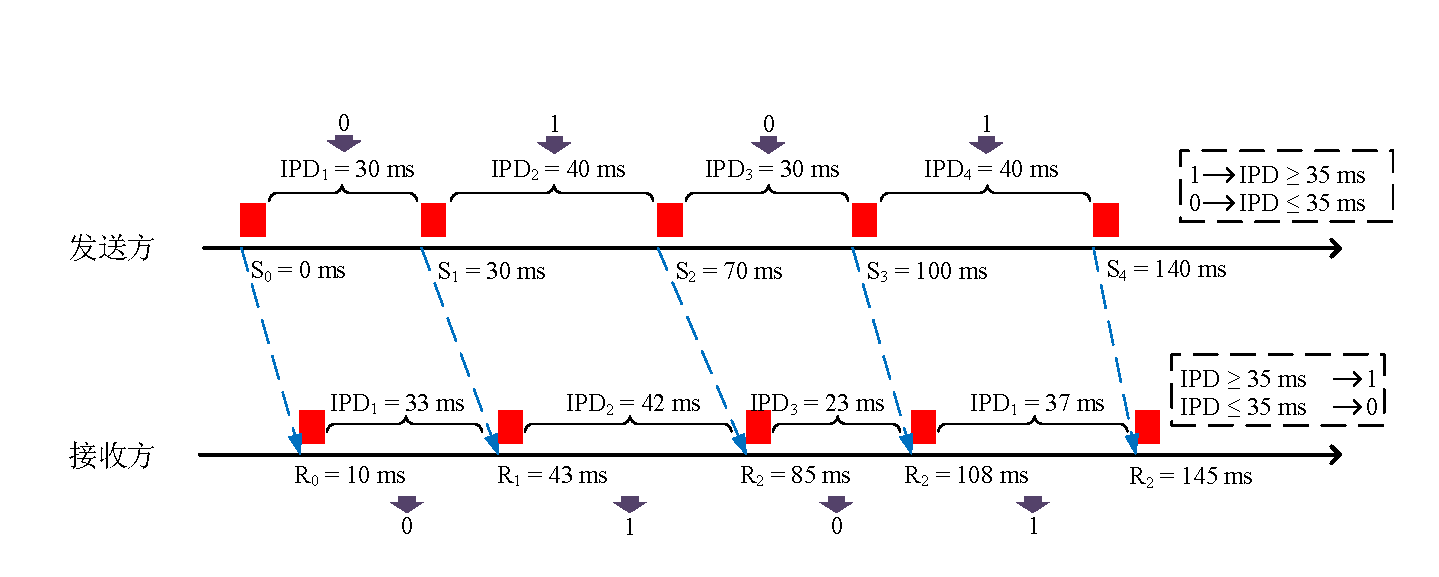
\includegraphics[width=0.99\textwidth]{chapters/chapter2/figures/ipd-ctc.pdf}
        \caption{基于IPD的时间隐通道示意图}\label{fig:2:ipd-ctc}
	\end{figure}
}

数据包的传输过程,存在传输时间间隔特征,利用该特征构建的时间隐通道,即为基于IPD的时间隐通道。\nupcite{4317620,8600755,WALLS20111217}如图\nref{fig:2:ipd-ctc},已知宿主信道的平均IPD为{35\ ms},待发送的二进制数据序列为$\{0,\ 1,\ 0,\ 1,\ \cdots\}$。对于发送方,当需要传输1时,将当前的IPD设定为{35\ ms}以上;当需要传输0时,将当前的IPD设定为{35\ ms}以内。图中根据数据包分布及消息内容,调整数据包发送时刻,实现隐通道调制。当数据包经网络传输后,噪声及传输调度导致IPD出现畸变。如果噪声太强,接收方使用相同的规则进行解调后,接收的隐蔽消息中将出现误码。

%on-off CTC
\insertFigure{
	\begin{figure}
		\centering
        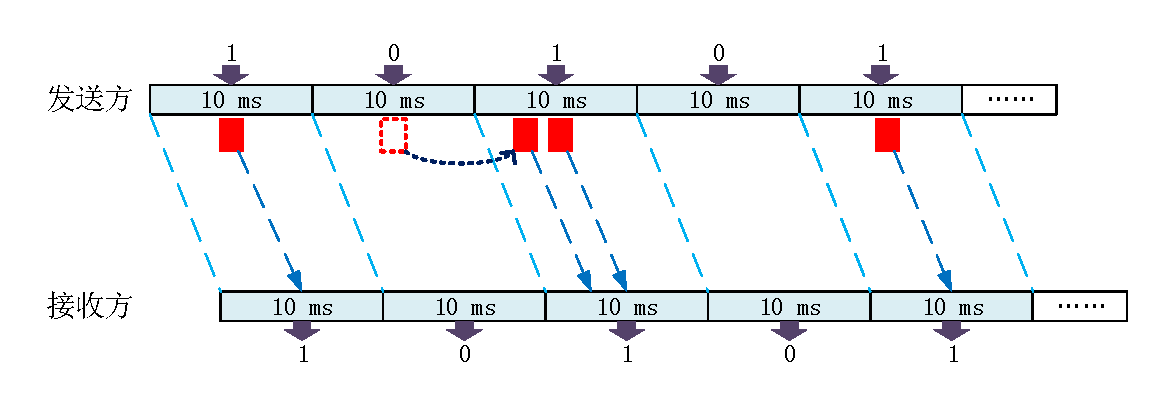
\includegraphics[width=0.9\textwidth]{chapters/chapter2/figures/onoff-ctc.pdf}
        \caption{基于On/Off模式的时间隐通道示意图}\label{fig:2:onoff-ctc}
	\end{figure}
}
另一种典型的时间隐通道为On/Off模式的时间隐通道,类似于开关的开关状态,通过控制是否传输数据包,调整任意时间段内的对应发送状态,完成时间隐通道构建。\nupcite{Cabuk:2004:ICT:1030083.1030108,5062145,6406084}如图\nref{fig:2:onoff-ctc},发送方与接收方设定{10\ ms}的时间窗口,控制在窗口内是否发送数据包,发送则代表传输1,不发送则代表传输0。在这类时间隐通道中,隐蔽消息编码适用不归零编码,双方利用时钟作为同步信号。

%Model-based CTC
\insertFigure{
	\begin{figure}
		\centering
        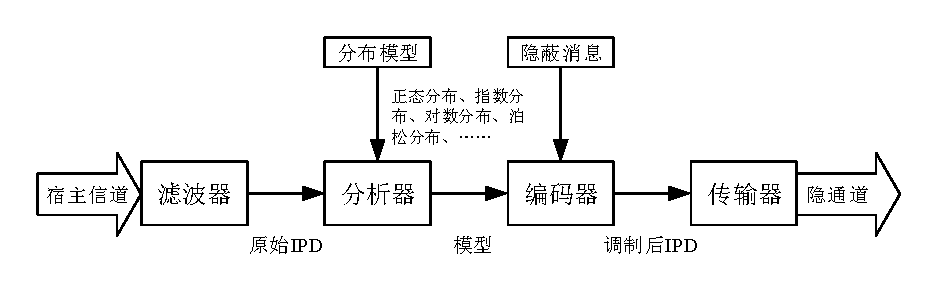
\includegraphics[width=0.85\textwidth]{chapters/chapter2/figures/mb-ctc.pdf}
        \caption{基于模型的时间隐通道示意图}\label{fig:2:mb-ctc}
	\end{figure}
}
基于模型的时间隐通道(MB-CTC),通过建模信道的传输特征,通过分布拟合的方式避免被监听者察觉。构建基于模型的时间隐通道,首先需要对拟合目标进行建模,创建拟合目标。\nupcite{5062145,ahsan2002practical}基于模型的时间隐通道调制器部分,通常包含滤波器、分析器、编码器及传输器几个部分,实现对传输特征的调整,完成隐通道构建。如图\nref{fig:2:mb-ctc},滤波器分析宿主信道中的IPD特征,并将分析结果传送给分析器。分析器根据已知的模型特征,分析当前适配的模型类型。编码器利用该模型,借助分布函数及累积分布函数,将隐蔽消息编码进IPD中。传输器根据目标IPD,调整数据包发送间隔,完成调制过程。

\subsection{基于移动互联网的时间隐通道构建方案}
\label{chap:backinfo:ctc:mobile}
%介绍Skype、VoIP等构建方案
移动互联网环境下的时间隐通道构建方法,与以太网环境下时间隐通道的构建原理存在相似点。但在移动互联网环境中,数据包传输特征发生了变化,基于以太网的时间隐通道构建方法不完全适用,尤其是隐蔽性方面难以满足需求。

\insertFigure{
	\begin{figure}
		\centering
        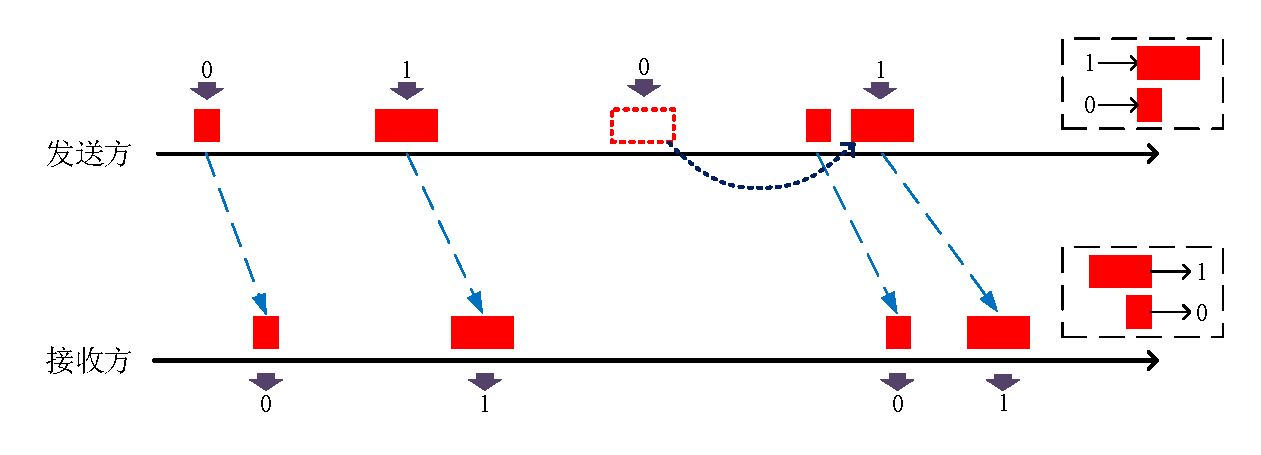
\includegraphics[width=0.95\textwidth]{chapters/chapter2/figures/pl-ctc.pdf}
        \caption{基于数据包长度的时间隐通道示意图}\label{fig:2:pl-ctc}
	\end{figure}
}

%Packet-Length CTC。 Liang
对于VoIP等实时交互应用,数据包长度并不是完全随机的,数据包长度根据传输需求不断变化,数据包长度是时间隐通道的有效载体。构建基于数据包长度的时间隐通道,首先统计数据包长度分布,划分长度区间并对应到编码符号。在发送过程中,根据待发送数据包的长度,以及当前的消息发送内容,通过调整数据包顺序完成隐蔽消息嵌入。\nupcite{LIANG2018144,8277839}如图\nref{fig:2:pl-ctc},通过调整数据包发送顺序,根据隐蔽消息内容构建数据包序列,即可构建基于数据包长度的时间隐通道。

%Packet-content CTC
移动互联网中的数据包,尤其是RTP数据包,在一次通话过程中的数据包内容唯一。因此,数据包自身也构成了连续不断的特征流,并且数据包内容出现HASH冲突的概率非常低。基于数据包内容的时间隐通道借助信息摘要算法,计算负载的摘要作为数据包标记。通过调整不数据包的位置,构建数据包标记序列,完成消息嵌入实现隐通道构建。\nupcite{LIANG2018162,6670985}

%VoLTE RTP、RTCP CTC
对于VoLTE,由于采用了基于RTP的传输方案,同时需要RTCP数据包完成传输反馈。这两种同时存在的数据包,在发送序列中形成了可观测的传输特征。由于RTCP数据包数量较少,并且发送过程比较离散,具有传输定位的功能。通过调整RTCP数据包之间的RTP数据包的数量,隐蔽消息被嵌入到RTP数据包数量中,接收方统计数据包数量即可还原隐蔽消息。\nupcite{ZHANG201866}

\insertFigure{
	\begin{figure}
		\centering
        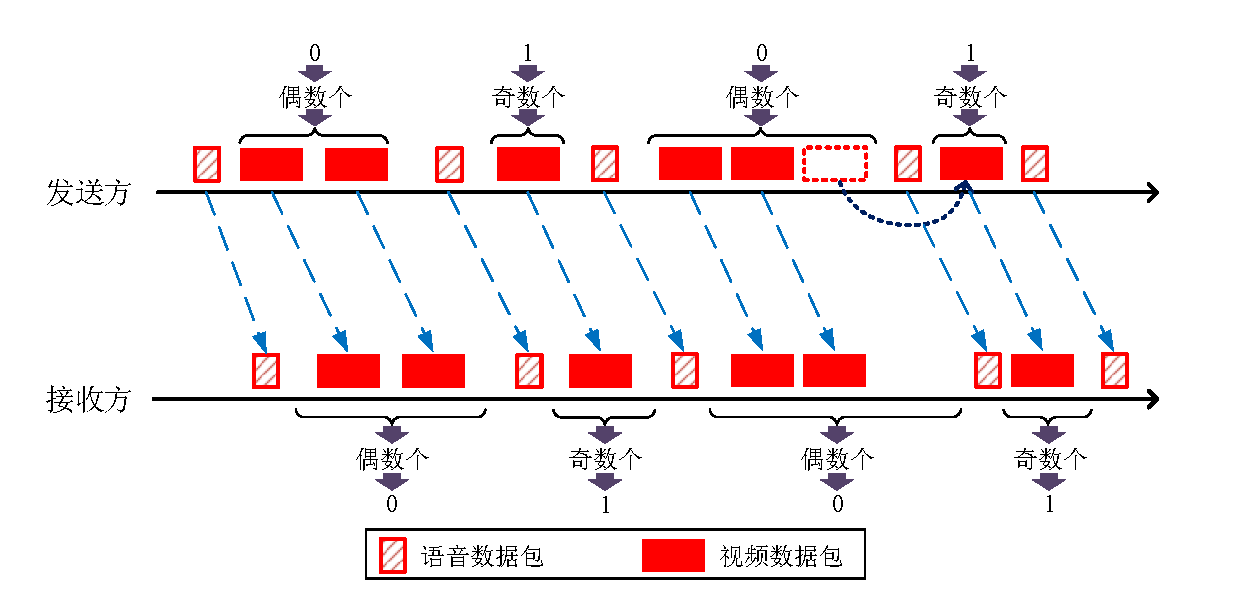
\includegraphics[width=0.9\textwidth]{chapters/chapter2/figures/av-ctc.pdf}
        \caption{基于数据包计数的时间隐通道示意图}\label{fig:2:av-ctc}
	\end{figure}
}

%VoLTE Video、Audio CTC
类似基于RTP及RTCP的时间隐通道\nupcite{ZHANG201866},基于语音数据包及视频数据包计数构建时间隐通道也是可行的。参考图\nref{fig:2:ap-bp},语音数据包及视频数据包最终都由BP进行处理。在BP侧,语音数据包具有明显的传输规律,具备参照时钟的功能。语音数据包之间的视频数据包数量,随时间段变化,采用{AMR-WB}语音编码时,语音数据包每{20\ ms}发送一次。另一方面,视频帧率为{30\ fps}时的采样周期大约为{33\ ms},导致视频数据包与语音数据包发送周期不同步。因此,调整语音数据包之间视频数据包数量的方法,符合传输隐蔽性的要求。该模式的示意图如图\nref{fig:2:av-ctc},由于调整的数据包数量少,具有良好的传输隐蔽性。

\subsection{时间隐通道的鲁棒性策略}
\label{chap:backinfo:ctc:robustness}
正如\nref{sec:intro:background:robustness}所述,时间隐通道在鲁棒性方面需要格外重视。隐通道中常用的鲁棒性方法,包括鲁棒性编码、附加校验及纠错信息等。不同的方法各有优势,在应用中通常结合噪声类型,根据去噪需求确定鲁棒性策略。

%介绍各个方案中,为保证鲁棒性,采用的检错、纠错编码,重传策略等
%Gray码
\insertTable{
	\begin{table}
        \centering
        \caption{格雷码编码表}
        \label{tab:2:gray-code}
        \begin{tabular*}{0.6\textwidth}{@{\extracolsep{\fill}}cccc}
        \toprule
        数据 & 1 bit格雷码 & 2 bit格雷码 & 3 bit格雷码\\ 
        \midrule
        0 & 0 & 00 & 000 \\ 
        1 & 1 & 01 & 001 \\ 
        2 &   & 11 & 011 \\ 
        3 &   & 10 & 010 \\ 
        4 &   &    & 110 \\ 
        5 &   &    & 111 \\ 
        6 &   &    & 101 \\ 
        7 &   &    & 100 \\ 
        \bottomrule
        \end{tabular*}
    \end{table}
}

\insertFigure{
	\begin{figure}
		\centering
        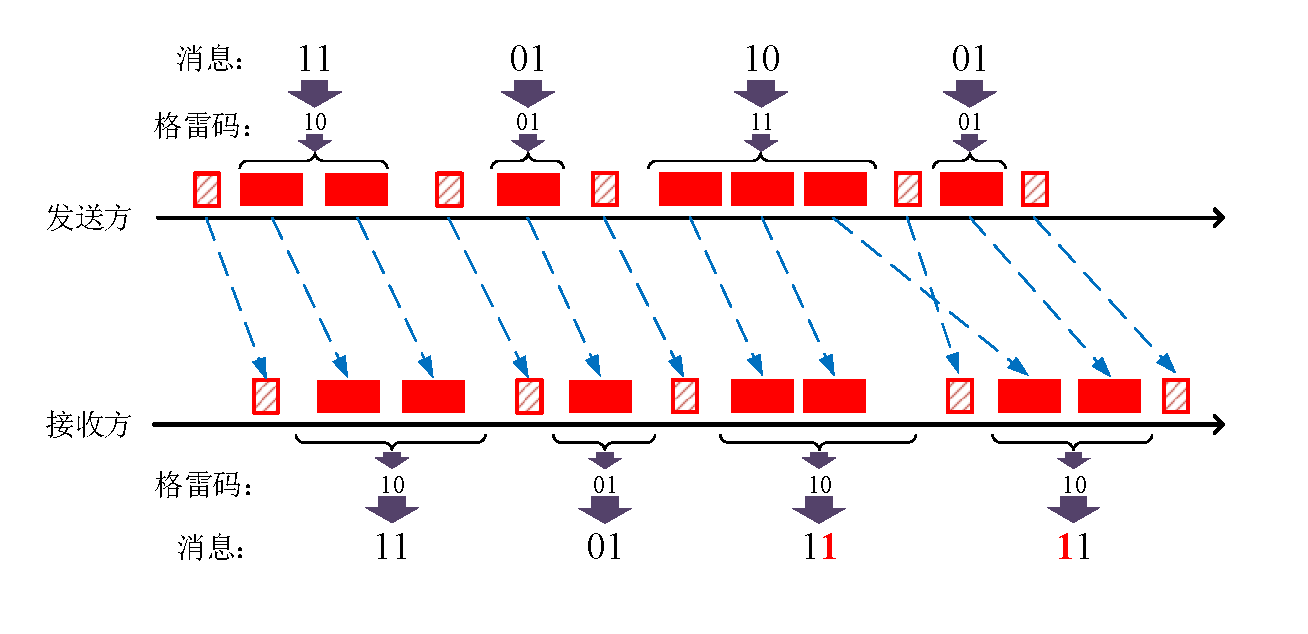
\includegraphics[width=0.9\textwidth]{chapters/chapter2/figures/gray-ctc.pdf}
        \caption{基于格雷码的时间隐通道鲁棒性示意图}\label{fig:2:gray-ctc}
	\end{figure}
}

格雷码又称循环二进制单位距离码,任意两个相邻数值的编码只有一个二进制位不同,与奇偶校验码同属于可靠性编码。\nupcite{7329924}不同位数的格雷码如表\nref{tab:2:gray-code}所示,利用相邻数据编码差异小的优势,当统计误差只有$\pm1$时,错误只影响一个二进制位,减少了误码的位数。格雷码的应用优势如图\nref{fig:2:gray-ctc},发送方使用数据包计数进行调制,接收过程中出现不可预期的乱序时,格雷码能够防止噪声扩散。\nupcite{8600755,8817935}

%Guard Band
受网络噪声的影响,编码符号之间的区分难度增大,需要在符号之间设定一定长度的隔离区,从而减弱噪声的干扰强度。当监测到的符号落入隔离区时,则视为噪声丢弃,否则处理后将产生显著的误码。根据符号的类型,隔离区设定为单个\nupcite{6567004,6296078},或设定为多个\nupcite{LIANG2018162},与符号的对应范围密切相关。

%喷泉码等
除了以上方法,一些特殊的编码算法,也应用在了时间隐通道中。基于喷泉码的时间隐通道,使用随机生成的关系矩阵,建立原始数据符号的线性编码。该方法保证了每个符号中有足够的冗余信息,结合抹除码的特征,在正确接收符号的前提下,具有较好的保密性和鲁棒性。\nupcite{6296078}除了喷泉码,低密度奇偶校验码、里所码、卷积码、Turbo码均在一定程度上提升了鲁棒性。\nupcite{10.1007/978-3-642-24178-9_22}

\subsection{基于主动丢包的时间隐通道研究要点}
在VoLTE场景中,存在的噪声只有丢包和乱序两种。基于主动丢包的时间隐通道,隐匿在丢包噪声中,构建方法的基本原理与现有方法存在区别。当前的时间隐通道鲁棒性策略,主要是抵御网络噪声的少量干扰。对于本文的时间隐通道构建方法,更重要的是将微弱的信号与背景噪声进行区分。由于解调过程无法确保正确性,可靠性编码不能完全解决该问题,需要设计一种内部交叉校验的鲁棒性方法。